\documentclass[11pt]{article}
\usepackage[T1]{fontenc}
\usepackage[utf8]{inputenc}
\usepackage[a4paper,margin=26mm]{geometry}
\usepackage{amsmath,amssymb,amsthm,mathtools,booktabs,array}
\usepackage{tikz}
\usetikzlibrary{arrows.meta,calc,positioning}
\usepackage[hidelinks]{hyperref}
\usepackage{xurl}
\newtheorem{theorem}{Theorem}[section]
\newtheorem{lemma}[theorem]{Lemma}
\newtheorem{proposition}[theorem]{Proposition}
\newtheorem{corollary}[theorem]{Corollary}
\newcommand{\HH}{\mathbb H}
\newcommand{\ip}[2]{\langle #1,#2\rangle}
\newcommand{\Pthree}{P_3}
\newcommand{\Qeight}{Q_8}
\newcommand{\EE}{\mathbb E}
\newcommand{\pos}[1]{(#1)_+}
\newcommand{\file}{\path}
\tikzset{finite/.style={circle,draw,fill=black,inner sep=2pt},
 ideal/.style={circle,draw,fill=white,inner sep=2.6pt},
 every picture/.style={line cap=round,line join=round}}
\title{A dimension bound of ten for right-angled hyperbolic polytopes}
\author{Coxeter Polytopes Frontier Project}
\date{20 October 2026; internal research manuscript}
\begin{document}
\maketitle
\begin{abstract}
We prove that a finite-volume right-angled hyperbolic polytope has
dimension at most ten. The new argument excludes the mixed case in
dimension eleven. Canonical three-faces define an undirected opposition
graph on finite vertices, with one invariant Lorentz vector and one
fixed null direction on each component. A structured positive-part
inequality, applied only to directions whose edges end ideally, gives
$2B\le84f+3E/2$. Here $B$ counts the canonical three-faces, $f$ the
finite vertices, and $E$ a nonnegative three-face excess. Polygon
incidences, a one-cusp exclusion and a balanced corner count give the
incompatible strict inequality $3722B>159195f+2794E$.
The geometric and counting arguments are given in full. The scalar
proof uses exact moment identities and finite rational positivity
certificates for seven, eight and ten directions. Published bounds for the compact
and entirely ideal cases, together with face heredity, give the
universal statement. A separate conditional Lean module checks the
final count logic; it does not formalize the hyperbolic geometry.
No new example or sharpness assertion is made.
\end{abstract}

\section{Statement and conventions}
\begin{theorem}\label{thm:main}
Every finite-volume right-angled hyperbolic polytope has dimension
at most ten.
\end{theorem}
We will exclude a polytope having both finite and ideal vertices in
$\HH^{11}$. Any higher-dimensional finite-volume right-angled polytope
has an eleven-dimensional face. Faces of dimension at least three inherit
right angles and finite volume: their finite and ideal links are faces of orthant and compact
cube links. The eleven-face cannot be compact or entirely ideal,
by the published upper bounds four and six~\cite{PV,Kolpakov}.
The exclusion therefore proves Theorem~\ref{thm:main} without using a
previous unrestricted dimensional bound.

Let $P\subset\HH^{11}$ be a hypothetical mixed polytope. Write $f>0$
for its finite vertices, $c>0$ for its ideal vertices, and $a_j$ for
its $j$-faces. We use Lorentz signature $(11,1)$, future unit points
$q^2=-1$, and outward unit normals $n$ with wall inequality
$\ip{x}{n}\le0$. Distinct outward normals have nonpositive products.
At a finite vertex the eleven incident normals are orthonormal;
direction $i$ omits normal $n_i$. Cusps are future null rays, and
their links are Euclidean ten-boxes. Two-faces have angles $\pi/2$
at finite vertices and zero at cusps.

Besides the two published dimension bounds, the external inputs are
the standard acute-wall/link facts, simple cusp truncation,
Dehn--Sommerville symmetry, and the published lower bound of $82$ on
the number of facets of a finite-volume right-angled eight-polytope~\cite[Sections 2--6]{Alex}.
The compact ceiling four makes every eight-face noncompact, so that
lower bound applies. No arithmetic or facet-spectrum hypothesis is used.

\section{Actual oppositions and a fixed null frame}
\begin{lemma}\label{lem:gap}
Distinct unit outward normals have product zero or at most $-1$.
\end{lemma}
\begin{proof}
Suppose their product $g$ lies in $(-1,0)$. Their Gram matrix
$G=\left(\begin{smallmatrix}1&g\\g&1\end{smallmatrix}\right)$
is positive definite and its inverse is entrywise nonnegative. For
a strict future interior point $x$, let
$b=(\ip{x}{u},\ip{x}{v})^T<0$ and
$x_0=x-[u\ v]G^{-1}b$. The coefficients added to $x$ are positive.
Acuteness therefore makes all other walls strict at $x_0$.
Also $x_0^2=x^2-b^TG^{-1}b<0$ and $\ip{x_0}{x}<0$.
Thus these walls meet along an actual ridge with a nonright angle,
a contradiction. The same projection argument applies to a larger
orthonormal set of actual walls.
\end{proof}

Call a triangular two-face with one finite and two ideal vertices a
\emph{bad triangle}. At $q$ make a graph on its eleven directions,
joining $i,j$ when their polygon is a bad triangle. The ideal
endpoints and the third wall are respectively
\begin{equation}\label{eq:bad}
 u_i=q-n_i,\qquad u_j=q-n_j,\qquad m_{ij}=q-n_i-n_j.
\end{equation}
These formulas follow from the edge null equations, incidence, unit
norm and the strict negative product of the third wall with $q$.

\begin{lemma}\label{lem:P3}
A triangle $S=\{i,j,k\}$ in this graph gives an actual three-face
$\Pthree$, a triangular bipyramid with two finite and three ideal
vertices. Its other finite vertex is
\begin{equation}\label{eq:move}
 q_S=2q-n_i-n_j-n_k.
\end{equation}
All six polygon facets of this three-face are bad triangles.
\end{lemma}
\begin{proof}
The three actual normals $m_{ij},m_{ik},m_{jk}$ are orthonormal.
The displayed $q_S$ is future unit timelike, is perpendicular to
these three normals and all $n_l$ outside $S$, and has strictly
negative products with $n_i,n_j,n_k$.
For any remaining wall write its normal in the complete frame as
$r=a q-\sum_l b_l n_l$, with $a>0$ and $b_l\ge0$.
Acuteness with the three $m$ walls gives
$b_i+b_j,b_i+b_k,b_j+b_k\le a$. Therefore
$\ip{r}{q_S}=-2a+b_i+b_j+b_k\le-a/2<0$.
This checks every wall, so $q_S$ is an actual finite vertex.

In the Lorentz four-space of this three-face the six known walls
are $y_l\ge0$ and $y_l+y_m\le t$ for
$x=tq-\sum_{l\in S}y_l n_l$. They enclose exactly the finite-volume
convex hull of $q,q_S,u_i,u_j,u_k$. The ideal points are feasible:
they are the actual endpoints of the three edges at $q$.
All five points lie in the closed chamber, so convexity prevents any
other wall from cutting this hull. This proves the assertion for
the whole three-face, not just its corner.
\end{proof}

\begin{figure}[ht]
\centering
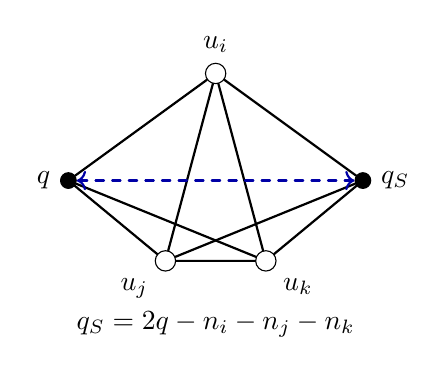
\begin{tikzpicture}[scale=.85]
 \node[finite,label=left:{$q$}] (q) at(-2.2,0){};
 \node[finite,label=right:{$q_S$}] (p) at(2.2,0){};
 \node[ideal,label=above:{$u_i$}] (i) at(0,1.6){};
 \node[ideal,label=below left:{$u_j$}] (j) at(-.75,-1.2){};
 \node[ideal,label=below right:{$u_k$}] (k) at(.75,-1.2){};
 \draw[thick] (i)--(j)--(k)--(i);
 \foreach \v in {i,j,k}{\draw[thick] (q)--(\v) (p)--(\v);}
 \draw[blue!65!black,thick,dashed,<->] (q)--(p);
 \node[align=center] at(0,-2.15)
 {$q_S=2q-n_i-n_j-n_k$};
\end{tikzpicture}
\caption{The actual $\Pthree$ three-face, drawn by incidence. Hollow
vertices are ideal; the dashed opposition is not a polytope edge.}
\label{fig:P3}
\end{figure}

Let $B$ count these three-faces. Each has two finite vertices and
gives one undirected opposition between them. Conversely the graph
triangle lemma identifies every opposition. Different triples at $q$
give different opposites by linear independence of its normals.
Thus the resulting graph on finite vertices has $B$ edges.
If $t(q)$ is its degree, then $\sum_q t(q)=2B$.

Across an opposition the new normals are the eight old normals outside
$S$ and the three $m$ normals. Their sum shows that
\begin{equation}\label{eq:invariant}
 h=3q-\sum_{i=1}^{11}n_i
 \quad\hbox{is invariant},\qquad h^2=2,\quad\ip{h}{q}=-3.
\end{equation}
On each connected component fix one nonzero future null vector
$Z\perp h$, possible because $h$ is spacelike. The same $Z$ is
used at both ends of every actual opposition. Define
\begin{equation}\label{eq:frame}
 F(q)=-\ip{Z}{q}>0,\qquad p_i=-\ip{Z}{n_i}/F(q).
\end{equation}
Decomposition $Z=F(q)(q-\sum_i p_i n_i)$ gives exactly
\begin{equation}\label{eq:constraints}
 \sum_{i=1}^{11}p_i=3,\qquad \sum_{i=1}^{11}p_i^2=1.
\end{equation}
Individual coordinates need not be positive. For any formal triple put
$r_S=2-\sum_{i\in S}p_i$. Centering the eleven coordinates at $3/11$
and applying Cauchy to a centered triple indicator gives
\begin{equation}\label{eq:r-range}
 \frac{13-4\sqrt3}{11}\le r_S\le\frac{13+4\sqrt3}{11},
 \qquad \frac{11}{20}<r_S<\frac{20}{11}.
\end{equation}
For an actual opposition, $r_S=F(q_S)/F(q)$ and the reverse ratio
is $r_S^{-1}$. Formal triples are not asserted to be actual faces.

\section{Three-face budgets}
For a finite-volume right-angled three-polyhedron write $F,s,p$ for
its facets, cusps and finite vertices, and $\nu=F+s$.
Finite and ideal degrees are three and four. Euler and polygon area give
\begin{equation}\label{eq:3Euler}
 p+2s=2F-4,\quad p+4s=2\nu-4,\quad
 \sum_{\text{polygons}}(u+2v-5)=F+2s-12\ge0.
\end{equation}
Here $u,v$ are a polygon's finite and ideal vertex counts. Each
summand is a nonnegative integer because its area is
$\pi(u+2v-4)/2>0$.

\begin{lemma}\label{lem:min3}
One has $F\ge6$ and $\nu\ge9$. Equality in either $F=6$ or
$\nu=9$ forces the whole polyhedron to be $\Pthree$.
\end{lemma}
\begin{proof}
The area row also gives $p+6s\ge20$. If $F\le5$, Euler gives
$p+2s\le6$, $s\le3$ and $p+6s\le18$, impossible.
For $F=6$, area gives $s\ge3$. The total polygon corners are
$24-2s$, so at least $2s$ of the six facets are triangles.
Thus $s\le3$, and $s=3,p=2$. All six facets are triangles, each
having at most one finite vertex. Their six finite corners force all
six to be bad. Lemma~\ref{lem:P3} identifies the polyhedron.
Finally $F\ge6$ and $F+2s\ge12$ imply $\nu\ge9$, with equality
only for $F=6,s=3$.
\end{proof}

\begin{lemma}\label{lem:attach}
Two bad triangular facets sharing an ideal--ideal edge force the
whole three-polyhedron to be $\Pthree$.
\end{lemma}
\begin{proof}
Normalize their shared future null endpoints $u,v$ by their products
$-1$ with the first finite apex. Its right angle gives $\ip{u}{v}=-1$.
Let $n_1,n_2$ be the two orthogonal triangle normals. The apices are
$q_1=u+v-n_2$ and $q_2=t u+t^{-1}v-n_1$, $t>0$:
the right angle makes the product of the null coefficients one,
and unit norm and orientation fix the normal coefficient $-1$.
The remaining four wall normals are
$u-n_2,v-n_2,t u-n_1,t^{-1}v-n_1$.
Two cross products are $-t,-t^{-1}$, so Lemma~\ref{lem:gap}
forces $t=1$. The point $w=u+v-n_1-n_2$ is future null and feasible:
it is the nonzero sum $(u-n_1)+(v-n_2)$ of actual outward normals;
acuteness checks every other wall and strict interior pairing fixes
its future orientation. The six walls enclose precisely the convex
hull of $q_1,q_2,u,v,w$. Convexity gives the whole polyhedron.
\end{proof}

\begin{lemma}\label{lem:small}
The noncanonical types with $\nu\le10$ are precisely the following
count patterns; metric uniqueness is unnecessary:
\[
\begin{array}{c|ccc|rrrr}
 &F&s&p&A_0&A_1&A_2&A_3\\\hline
 \Qeight&8&2&8&0&8&0&0\\
 R_7&7&3&4&1&0&3&0
\end{array}
\]
Here $A_j$ counts finite vertices with exactly $j$ ideal-ending edges.
\end{lemma}
\begin{proof}
At $\nu=10$, area gives $F\le8$, and $F=6$ is already canonical.
For $F=8,s=2$, all polygons have zero excess. A bad triangle would
have a zero-excess partner across its ideal edge, again a bad triangle,
contrary to Lemma~\ref{lem:attach}. There are no other triangles,
and the total of 32 polygon corners makes every facet a quadrilateral
with three finite and one ideal vertex. A finite vertex has at most
one ideal-ending edge. The two cusps have no mutual edge, so their
eight edges force exactly one at every finite vertex.

For $F=7,s=3,p=4$, the total excess is one and there are 24 polygon
corners. Hence at least four facets are triangles. Each ideal--ideal
edge has at most one bad triangular facet, and there are at most
three such edges, so at most three bad triangles occur. An all-ideal
triangle uses the one excess unit. It follows that there are exactly
three bad triangles, one ideal triangle, and three quadrilaterals
of type $(u,v)=(3,1)$. The ideal triangle uses all three ideal--ideal
edges, leaving six finite--ideal and three finite--finite edges.
No finite vertex has three ideal-ending edges: its three incident
polygons would be bad triangles, giving $\Pthree$.
The finite-edge graph on four vertices has three edges and no isolated
vertex. If it were a triangle and isolated vertex the latter would
have ideal degree three. It is therefore a tree. A path would have
ideal degrees $2,1,1,2$ and could support at most two bad triangles.
The tree must be a three-leaf star, with ideal degrees $0,2,2,2$.
\end{proof}

\begin{lemma}\label{lem:one-cusp}
A right-angled three-polyhedron with one cusp has at least eleven facets.
\end{lemma}
\begin{proof}
Equation~\eqref{eq:3Euler} gives $F\ge10$. If $F=10$, every polygon
has zero excess. The four facets at the cusp are quadrilaterals;
the other six are finite pentagons. Write the four quadrilaterals
cyclically as $Q_i=(u,A_i,B_i,A_{i+1})$, indices modulo four.
Opposite $Q_i$ have asymptotic planes meeting only at $u$, and each
$B_i$ belongs only to $Q_i$ among the four. Thus the eight finite
vertices displayed are distinct.
Let $P_i$ be the third facet at $A_i$. Its boundary contains
$B_{i-1}A_iB_i$. At $B_i$, the three facets are
$Q_i,P_i,P_{i+1}$, so consecutive $P_i$ are distinct and adjacent.
If $P_i=P_{i+2}$, its convex intersection with $P_{i+1}$ contains
both $B_i,B_{i+1}$ and is the edge joining them. The boundary of
$P_{i+1}$ would then be the triangle
$B_iA_{i+1}B_{i+1}$, impossible for a pentagon. Hence all four
$P_i$ are distinct and form four distinct pentagon adjacencies.

The eight quadrilateral--pentagon edges adjoin these four pentagons.
The remaining two pentagons $R,S$ adjoin no quadrilateral. Each
adjoins all five other pentagons, since two facets share at most one
edge. They give nine pentagon--pentagon edges, in addition to the
four among the $P_i$. But the pentagon degree count gives exactly
$(6\cdot5-8)/2=11$, contradicting at least thirteen.
\end{proof}

\begin{figure}[ht]
\centering
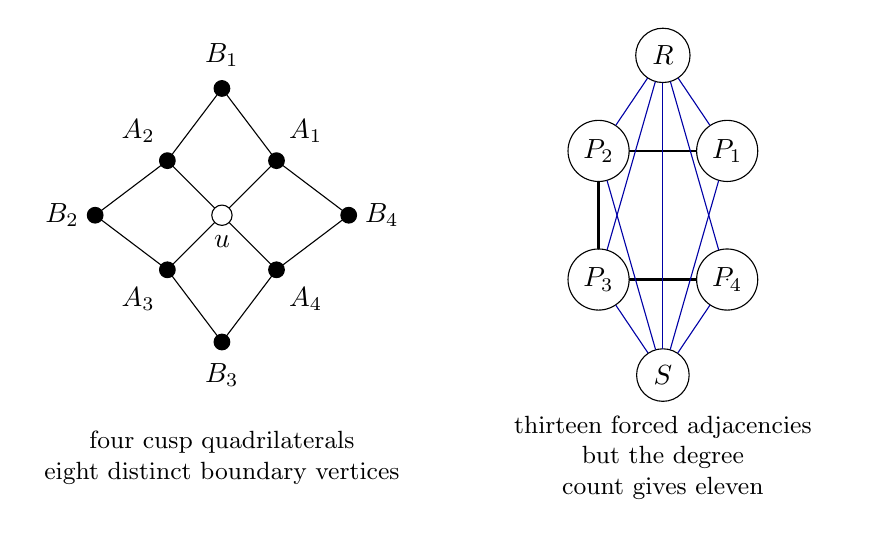
\begin{tikzpicture}[scale=.7]
 \coordinate (u) at(0,0);
 \foreach \i/\ang in {1/45,2/135,3/225,4/315}{
  \coordinate(A\i)at(\ang:1.4);
  \coordinate(B\i)at(\ang+45:2.3);
  \node[finite]at(A\i){};\node[finite]at(B\i){};
  \node at(\ang:2.15){$A_{\i}$};
  \node at(\ang+45:2.9){$B_{\i}$};
  \draw (u)--(A\i);}
 \node[ideal,label=below:{$u$}]at(u){};
 \draw(A1)--(B1)--(A2)--(B2)--(A3)--(B3)--(A4)--(B4)--cycle;
 \node[align=center,font=\small,text width=4.7cm]at(0,-4.4)
 {four cusp quadrilaterals\\eight distinct boundary vertices};
 \begin{scope}[xshift=8cm]
 \foreach \i/\ang in {1/45,2/135,3/225,4/315}{
  \node[circle,draw,inner sep=3pt](P\i)at(\ang:1.65){$P_{\i}$};}
 \draw[thick](P1)--(P2)--(P3)--(P4)--cycle;
 \node[draw,circle](R)at(0,2.9){$R$};
 \node[draw,circle](S)at(0,-2.9){$S$};
 \draw[blue!65!black](R)--(S);
 \foreach \i in {1,2,3,4}{\draw[blue!65!black](R)--(P\i)(S)--(P\i);}
 \node[align=center,font=\small,text width=4.7cm]at(0,-4.4)
 {thirteen forced adjacencies\\but the degree count gives eleven};
 \end{scope}
\end{tikzpicture}
\caption{The one-cusp equality obstruction. The right panel is a forced
facet-adjacency graph, not a planar embedding or a chamber realization.}
\label{fig:one-cusp}
\end{figure}

Call a three-face exceptional unless it is $\Pthree$ or $\Qeight$.
Define the nonnegative excess and signed defect
\begin{equation}\label{eq:ERdef}
 E=\sum_{Y\ne\Pthree}(\nu(Y)-10),\qquad
 R=\sum_{Y\ne\Pthree}(8-F(Y)).
\end{equation}
Let $X$ count exceptional finite-vertex/three-face incidences. Then
\begin{equation}\label{eq:Xbudget}
 X\le18E+4R.
\end{equation}
Indeed the right side of $p\le18(\nu-10)+4(8-F)$ minus $p$
is $20\nu-144-8F$. At $\nu=10$ the exceptional $R_7$ has equality.
At $\nu=11$, area gives $F\le10$ and Lemma~\ref{lem:one-cusp}
excludes $F=10$, leaving a positive difference. For $\nu\ge12$,
use $F\le\nu$. Both budgets vanish on $\Qeight$.

\begin{lemma}\label{lem:Hbudget}
With sums over actual three-faces, put
$D=\sum_Y(A_2(Y)-3A_0(Y))$ and
$H=\sum_{Y\ne\Pthree}A_3(Y)$. Then
\begin{equation}\label{eq:DH}
 D\ge-30E,\qquad H\le2E.
\end{equation}
\end{lemma}
\begin{proof}
All three small types have $A_2-3A_0=0$. At $\nu=11$,
Lemma~\ref{lem:one-cusp} and area give $F\le9$, hence $p\le10$.
For $\nu\ge12$, $p\le2\nu-4\le10(\nu-10)$.
Each remaining contribution to $D$ is at least $-3p$, proving its bound.

For the second bound, first take an all-ideal-edge finite corner in
a noncanonical three-face. Among its three incident polygons, every
one that is not a bad triangle has excess at least one. Across the
ideal edge of each bad triangle is another polygon. It is not a bad
triangle by Lemma~\ref{lem:attach}, so it too has excess at least one.
These opposite polygons are distinct and avoid the chosen corner:
their normals are the distinct $q-n_i-n_j$. There are thus three
distinct excess units, giving $F+2s\ge15$.
If $\nu\le10$, then $s\ge15-\nu$ and $4s\le2\nu-5$ are
incompatible. At $\nu=11$ they force $s=4,p=2$, so $A_3\le2$.
At $\nu=12$, $A_3\ge5$ would give $p\ge5$ and
$4s\ge3A_3\ge15$, hence $p+4s\ge21>20$ by integrality.
Thus $A_3\le4$. Finally $4A_3\le p+4s=2\nu-4$ gives
$A_3\le(\nu-2)/2\le2(\nu-10)$ for $\nu\ge13$.
Summation proves $H\le2E$ without a further metric classification.
\end{proof}

\section{The strict ordinary incidence lower bound}
At an ambient finite vertex let $k$ edges end ideally and put $m=11-k$.
Its contributions to $D,H$ are
$\binom{k}{2}m-3\binom m3$ and $\binom k3-t(q)$.
Every triple with zero or two ideal-ending directions is exceptional,
so $X(q)\ge\binom m3+\binom k2m$. The integer row
\[
 40\binom m3+28\binom k2m-16\left(165-\binom k3\right)\ge0
\]
has successive values
$3960,2160,972,288,0,0,180,432,648,720,540,0$ for $0\le k\le11$.
It follows pointwise and then by summation that
\begin{equation}\label{eq:Xlower}
 31X\ge16(165f-2B)+3D-16H
       \ge16(165f-2B)-122E.
\end{equation}
Together with~\eqref{eq:Xbudget}, this gives
$680E+124R\ge2640f-32B$.

Every polygon has nine three-cofaces, a finite vertex has 165,
and a cusp has $2^8\binom{10}{2}=11520$. Summing
$F=2+p/2+s$ and the definitions~\eqref{eq:ERdef} gives
\begin{align}
 a_3&=\frac92a_2-\frac{165}4f-5760c,\notag\\
 E&=B-10a_3+9a_2+11520c,\qquad
 R=8a_3-9a_2-2B.\label{eq:identities}
\end{align}

The strict weighted row needed below is
\begin{equation}\label{eq:weighted}
 a_2>\frac{25}2f+1930c.
\end{equation}
Here is its direct Dehn--Sommerville derivation. Simple truncation
has counts $b_0=f+1024c$, $b_{10}=a_{10}+c$ and
$b_k=a_k+2^{10-k}\binom{10}{k}c$ for $1\le k\le9$.
Symmetry of
$(t-1)^{11}+\sum_{k=0}^{10}b_k(t-1)^k$ gives
\begin{align*}
 f&=2a_6-12a_7+42a_8-112a_9+252a_{10}-252c-504,\\
 a_2&=25a_6-148a_7+515a_8-1370a_9+3080a_{10}-1220c-6160.
\end{align*}
For $\lambda=2123/1280$ these imply
\[
 55f+5120\lambda c-\frac{22}5a_2
 =-\frac{44}5a_7+44a_8-132a_9+308a_{10}-616<0.
\]
Indeed $4a_7\ge82a_8$ by the eight-face facet lower bound and
$2a_9\ge11a_{10}$ by the elementary ten-face facet minimum.
Both grouped pairs are nonpositive and the constant is strictly
negative. This proves~\eqref{eq:weighted}.

Eliminating $a_2,a_3$ in~\eqref{eq:identities} gives
\[
 R=-\frac54B-\frac{165}8f+5760c-\frac34E,\qquad
 360c<B-\frac{75}2f-E.
\]
Consequently $680E+124R\ge2640f-32B$ becomes
$587E-123B-10395f/2+714240c\ge0$.
Since $714240=1984\cdot360$, its left side is strictly less than
$1861B-159195f/2-1397E$. We have proved
\begin{equation}\label{eq:lower}
 \boxed{3722B>159195f+2794E.}
\end{equation}

\section{A structured scalar estimate}
The analytic input is proved by the subset cases below.
\begin{proposition}\label{prop:scalar}
Let eleven real numbers satisfy~\eqref{eq:constraints}, and let $I$
be any $k$-element subset. For $r_S=2-\sum_{i\in S}p_i$,
\begin{equation}\label{eq:contract}
 \sum_{\substack{S\subset I\\|S|=3}}\pos{r_S^{-2}-\frac{37}{100}}
 \le\frac{756}{25}+\frac{27}{100}\binom k3.
\end{equation}
\end{proposition}
Write $\lambda=37/100$ and $\rho=10/\sqrt{37}$.
For $3\le k<11$, set
\[
 S=\sum_Ip_i,\quad y_i=p_i-S/k,\quad V=\sum_Iy_i^2,
 \quad\mu=2-3S/k,\quad d_T=-\sum_{i\in T}y_i.
\]
Cauchy on the complement gives
\begin{equation}\label{eq:subsetV}
 0\le V\le v_k(S):=1-S^2/k-(3-S)^2/(11-k),\quad
 \frac{3k-\sqrt{2k(11-k)}}{11}\le S\le
 \frac{3k+\sqrt{2k(11-k)}}{11}.
\end{equation}
In particular $V\le2/11$. Uniform averages over the $\binom k3$
triples satisfy, with $T_j=\sum_I y_i^j$,
\begin{align}
 \EE d&=0,&\EE d^2&=\alpha_2V,&\EE d^3&=-\alpha_3T_3,
 &\EE d^4&=\alpha_4T_4+b_4V^2,\label{eq:moments}\\
 \alpha_2&=\frac{3(k-3)}{k(k-1)},&
 \alpha_3&=\frac{3(k-3)(k-6)}{k(k-1)(k-2)},\notag\\
 \alpha_4&=\frac{3(k^2-17k+54)}{k(k-1)(k-2)},&
 b_4&=\frac{18(k-4)}{k(k-1)(k-2)}.\notag
\end{align}
These follow by expanding products of indicators: the inclusion
probabilities of one, two and three specified indices are
$3/k$, $6/[k(k-1)]$ and $6/[k(k-1)(k-2)]$.
The fourth expansion uses
$\sum_{i\ne j}y_i^3y_j=-T_4$,
$\sum_{i<j}y_i^2y_j^2=(V^2-T_4)/2$, and
$\sum_i y_i^2\sum_{j<l,\ j,l\ne i}y_jy_l=T_4-V^2/2$.

Two useful moment bounds are
\begin{equation}\label{eq:joint}
 T_4\ge V^2/k+T_3^2/V,\qquad
 |T_3|\le\frac{k-2}{\sqrt{k(k-1)}}V^{3/2}.
\end{equation}
The first is the orthogonal projection of $(y_i^2)$ onto the vectors
$1$ and $y$; interpret it by continuity at $V=0$.
For the second, $y_i\le M=\sqrt{(k-1)V/k}$. Put $b=-M/(k-1)$.
Expanding $\sum_i(M-y_i)(y_i-b)^2\ge0$ bounds $T_3$ from above
by $(k-2)MV/(k-1)$; replace $y$ by $-y$ for the lower bound.

For $r=\mu+d>0$ the exact identity
\begin{equation}\label{eq:remainder}
 r^{-2}=\mu^{-2}-2d\mu^{-3}+3d^2\mu^{-4}-4d^3\mu^{-5}
       +\frac{4r+\mu}{\mu^5r^2}d^4
\end{equation}
follows by clearing denominators. The remainder factor decreases in
$r$. With $a=11/20$, it is at most
$K(\mu)=(4a+\mu)/(\mu^5a^2)$.
The positive part is recovered by
\begin{equation}\label{eq:clip}
 \EE\pos{r^{-2}-\lambda}=\EE r^{-2}-\lambda+
 \EE\pos{\lambda-r^{-2}}.
\end{equation}
The last correction is at most $27/400$ by~\eqref{eq:r-range}.
If $b=\rho-\mu>0$, concavity of $\lambda-r^{-2}$ above $\rho$
and $(d-b)_+\le d^2/(4b)$ give
\begin{equation}\label{eq:clipvariance}
 \EE\pos{\lambda-r^{-2}}\le\frac{\lambda^{3/2}\EE d^2}{2(\rho-\mu)}.
\end{equation}
Here $\lambda^{3/2}<113/500$ and $\rho>18/11$; the correction
vanishes when an upper bound on $r$ is at most $18/11$.

For $k\le5$, each summand in~\eqref{eq:contract} is less than
$121/36-37/100=673/225$, since $r>6/11$.
There are at most ten triples, giving a total below $756/25$.
For $k=6$, pair every triple with its complementary triple in $I$.
Their ratios sum to $4-S>18/11$, by~\eqref{eq:subsetV} and
$S\le(18+2\sqrt{15})/11<26/11$.
The function $(r^{-2}-\lambda)_+$ is convex and decreasing.
With both ratios $>6/11$, each pair is bounded by its values at
$6/11$ and $12/11$, namely $12461/3600$ in total.
There are ten pairs; $12461/360<891/25$, the required right side.
Empty triple sums need no separate interpretation. This proves all
cases $k\le6$.

\section{Seven, eight and eleven directions}
For $k=7,8$, the coefficients in~\eqref{eq:moments} have
$\alpha_3>0$, $\alpha_4<0$ and $b_4+\alpha_4/k>0$.
Use $|T_3|\le V^{3/2}$ and $T_4\ge V^2/k$ in
\eqref{eq:remainder}. The average reciprocal is at most
\begin{equation}\label{eq:78env}
 J_k(\mu,V)=\mu^{-2}+3\alpha_2V\mu^{-4}
 +4\alpha_3V^{3/2}\mu^{-5}
 +K(\mu)(b_4+\alpha_4/k)V^2.
\end{equation}
Every displayed term is nonnegative, increases with $V$ and decreases
with positive $\mu$. For clarity, we give the full rational interval
certificate contract used to bound this expression; no sampled frames
or floating-point inequalities are required.

The admissible $S$ intervals in~\eqref{eq:subsetV} are contained in
$[27/22,57/22]$ for $k=7$ and $[17/11,31/11]$ for $k=8$.
Split these enclosing intervals into closed intervals
$[j/1100,(j+1)/1100]$, with respectively
$1350\le j<2850$ and $1700\le j<3100$.
For each interval $[l,u]$ set
\[
 S_* =\min(u,\max(l,3k/11)),\quad
 V_* =v_k(S_*),\quad \mu_-=2-3u/k,\quad\mu_+=2-3l/k.
\]
This is the exact maximum of the concave quadratic $v_k$ on the
interval. If $V_*<0$ the interval is empty of admissible frames.
Otherwise evaluate~\eqref{eq:78env} at $(\mu_-,V_*)$, rounding
$\sqrt{V_*}$ upward to a multiple of $10^{-6}$.
The rounding is certified by integer squaring, not numerical tolerance.
Add the least of the following applicable correction bounds:
\[
 \frac{27}{400},\qquad
 \frac{(113/500)\alpha_2V_*}{2(18/11-\mu_+)}
 \quad(\mu_+<18/11),\qquad
 0\quad\left(\mu_++\sqrt{3(k-3)V_*/k}\le18/11\right).
\]
For the last test the square root is again rounded upward.
These bounds follow from~\eqref{eq:clipvariance} and the centered
triple indicator norm. The resulting rational number is strictly less
than
\begin{equation}\label{eq:78goal}
 \lambda+\frac{756/25+(27/100)\binom k3}{\binom k3}
\end{equation}
on every nonempty interval. The exact certificate records these
checks and their least gaps:
\begin{center}
\begin{tabular}{ccccc}\toprule
$k$&enclosing intervals&nonempty&empty&least gap greater than\\\midrule
7&1500&1498&2&$6/25$\\
8&1400&1386&14&$3/50$\\\bottomrule
\end{tabular}
\end{center}
The intervals cover the whole domain and the envelopes bound each
whole interval. Thus these finite rational inequalities prove
\eqref{eq:contract} for $k=7,8$.

For $k=11$, $\mu=13/11$, $V=2/11$ and
\[
 \EE d^2=24/605,\quad \EE d^3=-4T_3/33,\quad
 \EE d^4=7V^2/55-2T_4/55.
\]
Here $K(13/11)<5$, so first replace the whole nonnegative fourth
moment remainder by five times that moment. Then use the joint bound
in~\eqref{eq:joint}. The reciprocal average is at most
\[
 \mu^{-2}+\frac{3(24/605)}{\mu^4}
 +5\frac{15}{121}V^2+\frac{16T_3}{33\mu^5}-T_3^2.
\]
The sharp cubic bound gives $|T_3|\le18/(121\sqrt5)<1/15$.
For $C=16/(33\mu^5)>2/15$, the function $CT_3-T_3^2$
is increasing on $[-1/15,1/15]$, so it is at most $C/15-1/225$.
Equation~\eqref{eq:clipvariance} bounds the correction by
$(113/500)(24/605)/(2(5/11))$. The resulting positive-part mean is
\[
 \frac{273313374321407}{611561341462500}
 <\frac{2493}{5500}
 =\frac{756/25+(27/100)\cdot165}{165}.
\]
This proves the full-subset case by rational comparisons alone.

\section{Nine directions: a global analytic bound}
For a nine-element set $I$, write $\delta=3-S$. Equation
\eqref{eq:subsetV} gives
\[
 0\le\delta\le12/11,\quad \mu=1+\delta/3,\quad
 0\le V\le2\delta/3-11\delta^2/18\le2/11.
\]
We prove the stronger mean estimate
\begin{equation}\label{eq:nine}
 \EE\pos{r^{-2}-\lambda}\le\frac{63}{100}-\frac\delta{18}.
\end{equation}
The moments here are
$\EE d^2=V/4$, $\EE d^3=-3T_3/28$ and
$\EE d^4=5V^2/28-3T_4/28\le V^2/6$.
The cubic bound~\eqref{eq:joint} gives
\[
 \frac37T_3\le\frac{V^{3/2}}{2\sqrt2}
 \le\frac{V}{2\sqrt{11}}\le\frac V6.
\]
For the clipping correction, $\rho>18/11$ and $\mu\le15/11$
imply $b=\rho-\mu>3/11$. The elementary global inequality
\[
 (d-b)_+\le\frac{27d^4}{256b^3}
\]
follows by maximizing $(d-b)/d^4$ for $d>b$, at $d=4b/3$.
Using the tangent bound as in~\eqref{eq:clipvariance} gives
\[
 \pos{\lambda-r^{-2}}
 \le\frac{54d^4}{256\rho^3b^3}
 \le\frac{11^6}{128\cdot18^3}d^4\le3d^4.
\]
In~\eqref{eq:remainder}, $\mu\ge1$, $r>11/20$ give a remainder
coefficient at most $r^{-2}+4r^{-1}<1280/121$.
Combining these estimates, with their signs unchanged, yields
\begin{equation}\label{eq:nineenv}
 \EE\pos{r^{-2}-\lambda}+\lambda
 \le\mu^{-2}+\frac{3V}{4\mu^4}+\frac{V}{6\mu^5}
       +\frac{1643}{726}V^2.
\end{equation}
Put $x=\delta/3$, so $0\le x\le4/11$ and
$V\le v=x(4-11x)/2$. The right side increases with $V$.
After substituting $v$, the exact cleared difference is
\[
 (1+x)^5\left[1-\frac{x}{6}
 -\left((1+x)^{-2}+\frac{3v}{4(1+x)^4}
 +\frac{v}{6(1+x)^5}+\frac{1643}{726}v^2\right)\right]=x^2R(x),
\]
where
\[
 R(x)=\frac{233}{24}+\frac{275}{24}x+\frac{10}3x^2
 +\frac{x^3}6-\frac{x^4}6
 -\frac{1643}{2904}(4-11x)^2(1+x)^5.
\]
The first five terms are at least $233/24$ since $0\le x<1$.
The derivative of the last product without its coefficient is
$(4-11x)(1+x)^4(-2-77x)\le0$, so the product is at most 16.
Thus $R(x)\ge233/24-1643\cdot16/2904=635/968>0$.
This proves~\eqref{eq:nine}; multiplying by 84 gives
$1323/25=756/25+(27/100)\binom93$, as required.
Equality is possible only at $\delta=0$, when the nine coordinates
are $1/3$ and the other two zero. No interval certificate is needed
for this case.

\section{Ten directions: joint moments and rational polynomials}
Let $v$ be the omitted coordinate. The remaining ten have
\begin{equation}\label{eq:tenframe}
 \frac{3-2\sqrt5}{11}\le v\le\frac{3+2\sqrt5}{11},\quad
 \mu=\frac{11+3v}{10},\quad V=\frac{1+6v-11v^2}{10}.
\end{equation}
Their moments are
$\EE d^2=7V/30$, $\EE d^3=-7T_3/60$ and
$\EE d^4=3V^2/20-T_4/15$.
Set $w=\sqrt{21V/10}$, $a=\mu-w$, and
$\gamma=8/\sqrt{90}$. The triple range and the sharp cubic bound give
$a>11/20$ and $|T_3|\le L=\gamma V^{3/2}$.
The exact remainder and the joint fourth moment imply
\begin{equation}\label{eq:tenenv}
 \EE r^{-2}\le\mu^{-2}+\frac{7V}{10\mu^4}
 +\max_{|T|\le L}\left\{\frac{7T}{15\mu^5}
 +K\left(\frac{43V^2}{300}-\frac{T^2}{15V}\right)\right\},
 \quad K=\frac{4a+\mu}{\mu^5a^2}.
\end{equation}
At $V=0$ the bracket is zero. On the actual cubic domain the coefficient
of $K$ is nonnegative, because $43/300-\gamma^2/15=259/2700>0$.
This observation is essential when increasing $K$; its positive and
negative occurrences cannot be changed independently.

In fact $K<7$. For $v\ge0$, $\mu\ge11/10$, $a>11/20$ give
$K\le12000000/1771561<7$. For $v\le0$, $V\le1/10$ and
$V'\ge3/5$, so $a'=3/10-(21/20)V'/\sqrt{21V/10}<0$.
Hence $a\ge a(0)=(11-\sqrt{21})/10>16/25$.
Also $v>-1/6$ gives $\mu>21/20$. Consequently
$K<7220000000/1045529856<7$. The endpoint $V=0$ follows by
continuity. We may replace the whole $K$ in~\eqref{eq:tenenv} by seven.

For $v\le0$, the vertex $V/(2\mu^5)$ of the concave quadratic
is beyond $L$, since
$2\gamma\mu^5\sqrt V\le(8/15)(11/10)^5<1$.
Using $\gamma<17/20$ and $\sqrt V\le1/10+(5/2)V$ gives
\begin{equation}\label{eq:Jneg}
 J_- =\mu^{-2}+\frac{7V}{10\mu^4}
 +\frac{119V/3000+119V^2/120}{\mu^5}
 +\frac{1813}{2700}V^2.
\end{equation}
The clipping correction is zero, since
$\mu+w<39/25<41/25<\rho$.
For $v\ge0$, completing the square without constraining $T$ gives
\begin{equation}\label{eq:Jpos}
 J_+ =\mu^{-2}+\frac{7V}{10\mu^4}
       +\frac{301}{300}V^2+\frac{7V}{60\mu^{10}}.
\end{equation}
For $0\le v\le1/20$, one has $\mu\le223/200$,
$V\le509/4000$, $w<13/25$, and hence $\mu+w<327/200<41/25$;
the correction is again zero. On the rest of the domain,
\eqref{eq:clipvariance}, $\lambda^{3/2}<113/500$ and $\rho>41/25$
give the correction bound
\begin{equation}\label{eq:tencor}
 C_+\le\frac{791V}{30000(41/25-\mu)}.
\end{equation}
The denominator stays positive on the larger interval $[1/20,7/10]$.

The required positive-part mean is $261/500$, equivalently the
corrected reciprocal mean is at most $223/250$. Clearing the positive
denominators in~\eqref{eq:Jneg}--\eqref{eq:tencor} reduces this to
the positivity of three explicit rational polynomials:
\begin{align}
 P_-={}&\frac{223}{250}\mu^5-\mu^3-\frac7{10}V\mu
 -\frac{119}{3000}V-\frac{119}{120}V^2
 -\frac{1813}{2700}V^2\mu^5,\notag\\
 P_0={}&\frac{223}{250}\mu^{10}-\mu^8-\frac7{10}V\mu^6
 -\frac{301}{300}V^2\mu^{10}-\frac7{60}V,\notag\\
 P_c={}&(41/25-\mu)P_0-\frac{791}{30000}V\mu^{10}.
 \label{eq:tenpoly}
\end{align}
Here $\mu,V$ are the polynomials in~\eqref{eq:tenframe}.
The respective domains, all enclosing the appropriate actual domain,
are $[-7/50,0]$, $[0,1/20]$ and $[1/20,7/10]$.
Some outer points have $V<0$; only polynomial positivity, not a moment
interpretation, is asserted at these extraneous points.

For completeness the exact finite positivity certificate is as follows.
For a degree-$m$ rational polynomial $Q$, expand
$Q(l+(u-l)t)=\sum_{j=0}^m c_jt^j$. Its Bernstein coefficients are
\begin{equation}\label{eq:Bernstein}
 \beta_i=\sum_{j=0}^i c_j\frac{\binom ij}{\binom mj},\qquad
 Q(l+(u-l)t)=\sum_{i=0}^m\beta_i\binom mi t^i(1-t)^{m-i}.
\end{equation}
The basis is nonnegative and sums to one on $[0,1]$.
On each consecutive interval of length $1/1000$, every coefficient
computed from~\eqref{eq:tenpoly} and~\eqref{eq:Bernstein} is strictly
positive. The complete table of obligation sizes is
\begin{center}
\begin{tabular}{ccrr}\toprule
polynomial&domain&intervals&positive coefficients\\\midrule
$P_-$, degree 9&$[-7/50,0]$&140&1400\\
$P_0$, degree 14&$[0,1/20]$&50&750\\
$P_c$, degree 15&$[1/20,7/10]$&650&10400\\\bottomrule
\end{tabular}
\end{center}
Thus all 12550 coefficients prove positivity on all 840 closed
intervals. They are recorded exactly, with digests and least coefficients,
in the accompanying certificate; the independent replay recomputes
them from the three displayed polynomials. This completes the
ten-direction case, and hence Proposition~\ref{prop:scalar}.

\section{Actual-subset deletion and the contradiction}
At a finite vertex $q$, let $I$ consist of the $k$ directions whose
edges end ideally. Its $t(q)$ actual $\Pthree$ triples are a subset of
the $\binom k3$ formal triples in $I$. For each actual triple,
$r^{-2}-1\le(r^{-2}-37/100)_+-63/100$.
Inserting other formal triples is legitimate because the added terms
are nonnegative. Proposition~\ref{prop:scalar} therefore gives
\begin{equation}\label{eq:delete}
 \sum_{\text{actual }S}(r_S^{-2}-1)
 \le\frac9{25}(84-t(q))
       +\frac{27}{100}\left(\binom k3-t(q)\right).
\end{equation}
The last parenthesis counts actual noncanonical three-faces whose
finite corner has three ideal-ending edges. Summed over ordinary
finite vertices it is exactly $H$, not an arbitrary graph error.

\begin{figure}[ht]
\centering
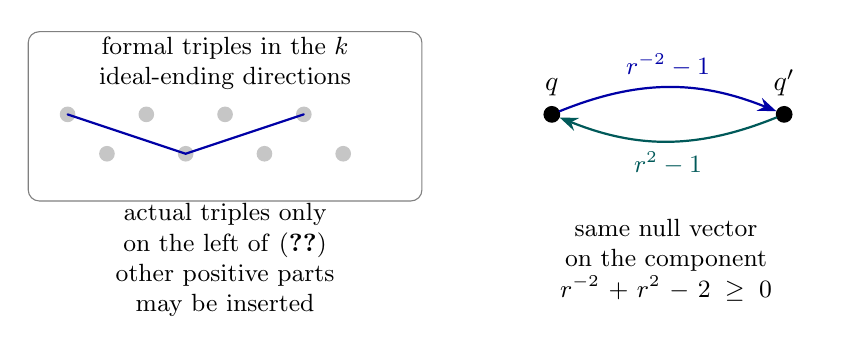
\begin{tikzpicture}[>=Stealth]
 \draw[rounded corners,gray](-5.5,-1.1)rectangle(-.5,1.05);
 \node[align=center,font=\small,text width=4.5cm]at(-3,.65)
 {formal triples in the $k$ ideal-ending directions};
 \foreach \x/\y in {-5/0,-4.5/-.5,-4/0,-3.5/-.5,-3/0,-2.5/-.5,-2/0,-1.5/-.5}
  \node[circle,fill=gray!45,inner sep=2pt]at(\x,\y){};
 \draw[blue!65!black,thick](-5,0)--(-3.5,-.5)--(-2,0);
 \node[font=\small,align=center,text width=4.6cm]at(-3,-1.85)
 {actual triples only on the left of~\eqref{eq:delete}\\other positive parts may be inserted};
 \node[finite,label=above:{$q$}](q)at(1.15,0){};
 \node[finite,label=above:{$q'$}](p)at(4.1,0){};
 \draw[->,thick,blue!65!black](q)to[bend left=22]
  node[above,font=\small]{$r^{-2}-1$}(p);
 \draw[->,thick,teal!70!black](p)to[bend left=22]
  node[below,font=\small]{$r^2-1$}(q);
 \node[align=center,font=\small,text width=4cm]at(2.6,-1.85)
 {same null vector on the component\\$r^{-2}+r^2-2\ge0$};
\end{tikzpicture}
\caption{Deletion and reversal use different domains. The scalar bound
enlarges an actual subset; the final sum pairs only actual opposition
edges. Neither panel asserts that formal triples are feasible faces.}
\label{fig:pairing}
\end{figure}

Sum~\eqref{eq:delete} over all finite vertices, with the fixed null
choice on each component. Every undirected opposition contributes
$r^{-2}+r^2-2=(r-r^{-1})^2\ge0$. As $\sum t=2B$ and $H\le2E$,
\[
 0\le\frac9{25}(84f-2B)+\frac{27}{100}H
 \le\frac9{25}(84f-2B)+\frac{27}{50}E.
\]
Consequently
\begin{equation}\label{eq:upper}
 \boxed{4B\le168f+3E.}
\end{equation}
This is an ordinary unweighted finite-vertex sum; it does not use a
maximum-height vertex or substitute a weighted average.

Twice~\eqref{eq:lower} and 1861 times~\eqref{eq:upper} say
\[
 7444B>318390f+5588E,\qquad
 7444B\le312648f+5583E.
\]
They would imply $5742f+5E<0$, contrary to $f>0$, $E\ge0$.
There is no mixed right-angled eleven-polytope. The eleven-face
argument in Section~1 proves Theorem~\ref{thm:main}.

\section*{Proof and verification record}
The proof separates universal geometry, exact incidence algebra and
finite scalar positivity. All local geometric arguments used by the
dimension exclusion are included above. Their independent written
reviews do not amount to external refereeing or full geometric
formalization. The only finite positivity supplements are the complete
seven/eight-direction rational interval envelopes and the three
ten-direction Bernstein polynomial obligations. They are interval
proofs, not a census of polytopes, a numerical search or sampled frames.

The exact standard-library checkers and compact certificates are:
\begin{itemize}
\item \file{scripts/check_mixed_eleven_balanced_and_subset_rows_20261020.py},
with \file{results/mixed_eleven_balanced_and_subset_rows_20261020.json};
\item \file{scripts/check_mixed_eleven_nine_direction_global_20261020.py},
with \file{results/mixed_eleven_nine_direction_global_20261020.json};
\item \file{scripts/check_mixed_k10_rational_envelopes_20261020.py},
with \file{results/right_angled_mixed_k10_rational_envelopes_20261020.json}.
\end{itemize}
Each has passed generation and a separate read-only exact replay.
The certificate archive stores the rational gaps, complete coefficient
digests, source bindings and bounded execution ledgers. An older
nine-direction interval certificate is preserved as independent support;
the global proof in Section~7 is sufficient here.

The standard-library module
\file{formal/CoxeterProofs/RightAngledMixed10.lean} has compiled in a
single capped batch and passed a separate printed-axiom audit.
Its primitive count identities, strict weighted row and three-face
budgets are explicit premises. It derives the balanced lower bound;
the summed real analytic transport inequality is a separate explicit
premise. From those inputs it checks the upper bound and contradiction,
and records the eleven-face dimensional tail as an interface.
The eight audited theorems use only \texttt{propext} and
\texttt{Quot.sound}; the integer comparison is axiom-free and there
is no \texttt{sorryAx}. The actual-wall geometry and the scalar-to-frame
interpretation remain written arguments, rather than hidden published
axioms or claims of end-to-end Lean verification.

\begin{thebibliography}{9}
\bibitem{PV} L. Potyagailo and E. Vinberg,
\emph{On right-angled reflection groups in hyperbolic spaces},
Commentarii Mathematici Helvetici \textbf{80} (2005),63--73.
\url{https://ems.press/content/serial-article-files/43032}.
\bibitem{Kolpakov} A. Kolpakov,
\emph{On the optimality of the ideal right-angled 24-cell},
Algebraic \& Geometric Topology \textbf{12} (2012),1941--1960.
\url{https://msp.org/agt/2012/12-4/agt-v12-n4-p03-s.pdf}.
\bibitem{Alex} S. Alexandrov,
\emph{On ideal vertices of right-angled hyperbolic polyhedra},
2023, Sections 2--6.
\url{https://arxiv.org/html/2303.09533v1}.
\end{thebibliography}
\end{document}
